%这个是根据计算机学报官网下的LaTeX模板改的,主要修改内容:①把GBK编码改成了UTF-8编码。②引入zhwinfonts,用上传的字体文件实现了字体的使用。
%现存的问题:①中文无法使用加粗功能,但是英文可以。解决方式1:使用黑体来凑合代替。解决方式2:在PDF编辑器里面一个一个加粗。②无法实现模板中所要求的每页脚注从1开始的要求。
%如果您在使用该模板的过程中遇到问题,或者有对该模板的修改意见,请联系本人:微信PolarisRisingWar(诸神缄默不语),或者CSDN诸神缄默不语(PolarisRisingWar)

\documentclass[10.5pt,compsoc]{CjC}
\usepackage{CJKutf8}
%\usepackage{CJK}
\usepackage{graphicx}
\usepackage{footmisc}
\usepackage{subfigure}
\usepackage{url}
\usepackage{multirow}
\usepackage[noadjust]{cite}
\usepackage{amsmath,amsthm}
\usepackage{amssymb,amsfonts}
\usepackage{booktabs}
\usepackage{color}
\usepackage{ccaption}
\usepackage{booktabs}
\usepackage{float}
\usepackage{fancyhdr}
\usepackage{caption}
\usepackage{xcolor,stfloats}
\usepackage{comment}
\setcounter{page}{1}
\graphicspath{{figures/}}
\usepackage{cuted}%flushend,
\usepackage{captionhack}
\usepackage{epstopdf}
\usepackage[utf8]{inputenc}
%\usepackage{ccmap}
%\CJKtilde
%\usepackage{CJKpunct} 
%\usepackage[lite,subscriptcorrection,slantedGreek,nofontinfo]{mtpro2}

%===============================%

%\firstfootname{ \quad \quad }
\headevenname{\mbox{\quad} \hfill  \mbox{\zihao{-5}{\begin{CJK*}{UTF8}{song}计\quad \quad 算\quad \quad 机\quad \quad 学\quad \quad 报\end{CJK*}} \hspace {50mm} \mbox{\begin{CJK*}{UTF8}{song}2019 年\end{CJK*}}}}%
\headoddname{\begin{CJK*}{UTF8}{song}? 期 \hfill
作者姓名等:论文题目\end{CJK*}}%

%footnote use of *
\renewcommand{\thefootnote}{\fnsymbol{footnote}}
\setcounter{footnote}{0}
\renewcommand\footnotelayout{\zihao{5-}}

\newtheoremstyle{mystyle}{0pt}{0pt}{\normalfont}{1em}{\bf}{}{1em}{}
\theoremstyle{mystyle}
\renewcommand\figurename{figure~}
\renewcommand{\thesubfigure}{(\alph{subfigure})}
\newcommand{\upcite}[1]{\textsuperscript{\cite{#1}}}
\renewcommand{\labelenumi}{(\arabic{enumi})}
\newcommand{\tabincell}[2]{\begin{tabular}{@{}#1@{}}#2\end{tabular}}
\newcommand{\abc}{\color{white}\vrule width 2pt}
\makeatletter
\renewcommand{\@biblabel}[1]{[#1]\hfill}
\makeatother
\setlength\parindent{2em}
%\renewcommand{\hth}{\begin{CJK*}{UTF8}{zhhei}}
%\renewcommand{\htss}{\begin{CJK*}{UTF8}{song}}

\input{zhwinfonts}
\begin{document}
\hyphenpenalty=50000
\makeatletter
\newcommand\mysmall{\@setfontsize\mysmall{7}{9.5}}
\newenvironment{tablehere}
  {\def\@captype{table}}

\let\temp\footnote
\renewcommand \footnote[1]{\temp{\zihao{-5}#1}}


\thispagestyle{plain}%
\thispagestyle{empty}%
\pagestyle{CjCheadings}

\begin{table*}[!t]
\vspace {-13mm}
\begin{tabular}{p{168mm}}
\zihao{5-}\begin{CJK*}{UTF8}{song}
第??卷\quad 第?期 \hfill 计\quad 算\quad 机\quad 学\quad 报\hfill Vol. ??  No. ?\end{CJK*}\\
\zihao{5-}\begin{CJK*}{UTF8}{song}
20??年?月 \hfill CHINESE JOURNAL OF COMPUTERS \hfill ???. 20??\end{CJK*}\\
\hline\\[-4.5mm]
\hline\end{tabular}

\centering
\vspace {11mm}
\begin{CJK*}{UTF8}{zhhei}
{\zihao{2} 题目(中英文题目一致)字体为2号黑体(全文除特别声明外, 外文统一用Times New Roman) }
\end{CJK*}
\vskip 5mm

{\zihao{3}\begin{CJK*}{UTF8}{fs}
作者名$^{1)}$\quad  作者名$^{2),3)}$ \quad 作者名$^{3) }$($^*$字体为3号仿宋*作者)\end{CJK*}}

\vspace {5mm}
\zihao{6}{\begin{CJK*}{UTF8}{song}
$^{1)}$(单位全名 部门(系)全名, 市(或直辖市) 国家名 邮政编码)
*字体为6号宋体*单位
\end{CJK*}}

\zihao{6}{\begin{CJK*}{UTF8}{song}
$^{2)}$(单位全名 部门(系)全名, 市(或直辖市) 国家名
邮政编码)*中英文单位名称、作者姓名须一致*
\end{CJK*}}

\zihao{6}{\begin{CJK*}{UTF8}{song}
$^{3)}$(单位全名 部门(系)全名, 市(或直辖市) 国家名 邮政编码)
\end{CJK*}}

\zihao{6}{\begin{CJK*}{UTF8}{zhhei}
论文定稿后,作者署名、单位无特殊情况不能变更。若变更,须提交签章申请,国家名为中国可以不写,省会城市不写省的名称,其他国家必须写国家名。
\end{CJK*}}

\vskip 5mm
{\centering
\begin{tabular}{p{160mm}}
\zihao{5-}{
\setlength{\baselineskip}{16pt}\selectfont{
\noindent\begin{CJK*}{UTF8}{zhhei}摘\quad 要\quad \end{CJK*} \begin{CJK*}{UTF8}{song}
*中文摘要内容置于此处(英文摘要中要有这些内容),字体为小5号宋体。摘要贡献部分,要有数据支持,不要出现``...大大提高''、``...显著改善''等描述,正确的描述是``比{\ldots}提高X{\%}''、
``在{\ldots}上改善X{\%}''。*摘要

\end{CJK*}\par}}\\[2mm]

\zihao{5-}{\noindent
\begin{CJK*}{UTF8}{zhhei}关键词\end{CJK*} \quad \begin{CJK*}{UTF8}{song}{*关键词(中文关键字与英文关键字对应且一致,应有5-7个关键词);关键词;关键词;关键词*  }
\end{CJK*}
}\\[2mm]
\zihao{5-}{\begin{CJK*}{UTF8}{zhhei}中图法分类号\end{CJK*}	\begin{CJK*}{UTF8}{song}
TP\end{CJK*}\rm{\quad \quad \quad     }
\begin{CJK*}{UTF8}{zhhei}DOI号:\end{CJK*}\begin{CJK*}{UTF8}{song}
*投稿时不提供DOI号\end{CJK*}}
\end{tabular}}

\vskip 7mm

\begin{center}
\zihao{3}{ {\begin{CJK*}{UTF8}{zhhei}Title *(中英文题目一致)字体为4号Times New Roman,加粗* Title\end{CJK*}}}\\
\vspace {5mm}
\zihao{5}{ {\begin{CJK*}{UTF8}{zhhei}NAME Name-Name$^{1)}$ NAME Name$^{2)}$ NAME Name-Name$^{3)}$ *字体为5号Times
new Roman*Name\end{CJK*}
}}\\
\vspace {2mm}
\zihao{6}{\begin{CJK*}{UTF8}{zhhei}{$^{1)}$(Department of ****, University, City ZipCode, China) *字体为6号Times
new Roman* Depart.Correspond}\end{CJK*}}

\zihao{6}{\begin{CJK*}{UTF8}{zhhei}{$^{2)}$(Department of ****, University, City ZipCode)*中国不写国家名*}\end{CJK*}}

\zihao{6}{\begin{CJK*}{UTF8}{zhhei}{$^{3)}$(Department of ****, University, City ZipCode, country)*外国写国家名*}\end{CJK*}}



\end{center}

\begin{tabular}{p{160mm}}
\zihao{5}{
\setlength{\baselineskip}{18pt}\selectfont{
{\bf Abstract}\quad \begin{CJK*}{UTF8}{zhhei}(\textbf{500英文单词,内容包含中文摘要的内容}).
字体为Times new Roman,字号5号* Abstract\end{CJK*}
\par}}\\

\setlength{\baselineskip}{18pt}\selectfont{
\zihao{5}{\noindent Do not modify the amount of space before and after the artworks. One- or two-column format artworks are preferred. and Tables, create a new break line and paste the resized artworks where desired. Do not modify the amount of space before and after the artworks. One- or two-column format artworks are preferred. All Schemes, Equations, Figures, and Tables should be mentioned in the text consecutively and numbered with Arabic numerals, and appear below where they are mentioned for the first time in the main text. To insert Schemes, Equations, Figures, and Tables, create a new break line and paste the resized artworks where desired. Do not modify the amount of space before and after the artworks. One- or two-column format artworks are preferred.Do not modify the amount of space before and after the artworks. One- or two-column format artworks are preferred. and Tables, create a new break line and paste the resized artworks where desired. Do not modify the amount of space before and after the artworks. One- or two-column format artworks are preferred. All Schemes, Equations, Figures, and Tables should be mentioned in the text consecutively and numbered with Arabic numerals, and appear below where they are mentioned for the first time in the main text.

\vspace {5mm}
{\bf Keywords}\quad \begin{CJK*}{UTF8}{zhhei}中文关键字与英文关键字对应且一致,\textbf{不要用英文缩写});
key word; key word; key word* *字体为5号Times new Roman * Key words\end{CJK*}}\par}
\end{tabular}

\setlength{\tabcolsep}{2pt}
\begin{tabular}{p{0.05cm}p{16.15cm}}
\multicolumn{2}{l}{\rule[4mm]{40mm}{0.1mm}}\\[-3mm]
&\begin{CJK*}{UTF8}{song}
收稿日期:\quad \quad -\quad -\quad ;最终修改稿收到日期:\quad \quad -\quad -\quad .*投稿时不填写此项*. 本课题得到… …基金中文完整名称(No.项目号)、… …基金中文完整名称(No.项目号)、… … 基金中文完整名称(No.项目号)资助.作者名1(通信作者),性别,xxxx年生,学位(或目前学历),职称,是/否计算机学会(CCF)会员(提供会员号),主要研究领域为*****、****.E-mail: **************.作者名2(通信作者),性别,xxxx年生,学位(或目前学历),职称,是/否计算机学会(CCF)会员(提供会员号),主要研究领域为*****、****.E-mail: **************. 作者名3(通信作者),性别,xxxx年生,学位(或目前学历),职称,是/否计算机学会(CCF)会员(提供会员号),主要研究领域为*****、****.E-mail: **************.(给出的电子邮件地址应不会因出国、毕业、更换工作单位等原因而变动。请给出所有作者的电子邮件)
第1作者手机号码(投稿时必须提供,以便紧急联系,发表时会删除): … …, E-mail: … …*此部分6号宋体*
\end{CJK*}
\end{tabular}\end{table*}
\clearpage\clearpage
\begin{strip}
\vspace {-13mm}
\end{strip}
    \linespread{1.15}
    \begin{CJK*}{UTF8}{zhhei}
\zihao{5}
\vskip 1mm
\section{方法}
LLM 对于不同格式的表格输入有着不同的响应,与自然语言加特定分隔符(NL+Sep)相比,使用 HTML 等标记语言更能提升模型性能 。进一步研究表明,自我增强提示法能帮助LLM 自我检索和利用内部知识,更好地理解表格数据的结构和语义 \cite{ref1}。

{\begin{CJK*}{UTF8}{zhhei}\subsection{one-shot}\end{CJK*}}

在 LLM 处理表格数据的场景下,one-shot 学习方法凭借其独特优势成为高效处理数据的重要策略。不同于需要大量标注数据的传统方法,one-shot 仅依赖单个示例,通过精准设计的提示模板,引导 LLM 基于已有知识和内部表征快速捕捉表格结构与语义特征。


{\begin{CJK*}{UTF8}{zhhei}\subsection{基于HTML标记语言的输入设计策略}\end{CJK*}}
在处理表格数据时,输入格式对 LLM 的理解和处理能力有着显著影响。自然语言加特定分隔符(NL+Sep)的方式虽然能提供一定的信息,但缺乏对表格结构的清晰表达,使得 LLM 在解析表格时可能出现信息丢失或理解偏差。而 HTML 标记语言具有丰富的标签系统,如 \texttt{<table>}、\texttt{<tr>}、\texttt{<td>} 等,能够精确地定义表格的结构。这种结构化的表示方式与 LLM 在训练过程中接触到的大量网页数据相契合,使得模型能够更直观地理解表格的层次结构和数据关系,从而提升处理表格数据的性能。

{\begin{CJK*}{UTF8}{zhhei}\subsection{自我增强提示法}\end{CJK*}}
LLM 虽具备强大的语言理解与生成能力,但处理复杂表格数据时,难以充分挖掘潜在信息。现有方法如思维链(CoT)提示法,主要是提供中间推理步骤示例辅助推理,在表格数据处理场景存在局限。它依赖自然语言描述推理步骤,易丢失表格结构细节,且性能提升受模型规模影响大,小模型难以有效利用,灵活性也欠佳,难以适应表格多样的结构和任务需求。
自我增强提示法核心是借助分阶段提示策略,让 LLM 自我检索和运用内部知识,提升对表格结构和语义的理解。


\section{实验}
本部分实验采用QWen2.5-7B-instruct进行测试,并预先制定了以下系统提示词:
\begin{verbatim}
You are an accurate table Q&A assistant. 
Please  carefully analyze the following
table and answer the questions 
accurately.
Note: Only output the answers,
do not explain the process.
"table_text": table content;
"statement": question.
Please give the answer directly.
\end{verbatim}

\begin{table}[htbp]
\centering 
\caption{Qwen2.5-7B-Instruct不同方法性能对比}
\label{tab:full_performance}
\vspace{-2.5mm}
\begin{center}
\begin{tabular}{lcccc}
\toprule
\textbf{方法} & \textbf{ACC} & \textbf{测试样本数} & \textbf{测试次数}  \\
\midrule
Zero-shot & 47.7\% & 100 & 5  \\
One-shot & 49.6\% & 100 & 5 &  \\
HTML标记语言 & 50.6\% & 100 & 5  \\
One-shot+HTML & 48.7\% & 100 & 5  \\
Self-augmented & 51.6\% & 100 & 5  \\
\bottomrule
\end{tabular}
\end{center}
\end{table}

{\begin{CJK*}{UTF8}{zhhei}\subsection{one-shot}\end{CJK*}}
见表\ref{tab:full_performance},one-shot的提升相比于zero-shot提升了1.9个百分点,达到49.6\%的准确率。这表明向模型提供一个示例能够有效改善其表格理解和问答能力。通过一个范例,模型可以更好地把握问题解答的格式和思路,从而提高回答的准确性。然而,提升幅度有限,说明单一示例可能不足以完全引导模型理解复杂表格结构和关系的分析方法。

{\begin{CJK*}{UTF8}{zhhei}\subsection{基于HTML标记语言的输入}\end{CJK*}}
见表\ref{tab:full_performance},基于HTML标记语言的输入方法将准确率提升至50.6\%,比zero-shot方法高出2.9个百分点,是单一方法中表现最好的。HTML结构化标记帮助模型更清晰地理解表格的层次关系和数据组织方式,为表格问答提供了更明确的结构信息。值得注意的是,同时采用了one-shot和HTML输入的方法反而导致性能下降至48.7\%,低于单独使用HTML标记的效果,这可能是由于两种方法结合产生了信息冗余或指导方向不一致所导致的干扰。

{\begin{CJK*}{UTF8}{zhhei}\subsection{自我提示增强}\end{CJK*}}
见表\ref{tab:full_performance},自我提示增强方法取得了最佳效果,准确率达到51.6\%,比基准zero-shot方法提升了3.9个百分点。该方法通过让模型首先进行自我思考,生成解题步骤和推理过程,然后再给出最终答案,有效提高了问题理解和推理的质量。这种"思考-回答"的两阶段机制使模型能够更全面地分析表格数据和问题要求,减少了直接跳到结论可能带来的错误。实验结果表明,引导模型进行结构化思考是提升表格问答任务性能的有效策略。表\ref{tab:model-usage-acc}给出的实验结果指出,比较集中在自增强提示词的设计上——实验结果表明,相较于简略提示,结构化且包含明确分步骤指引的详细提示词能够显著提升模型在表格理解和关键信息抽取任务中的表现,这一现象很可能与 Instruct 版本模型对指令敏感、擅长遵循多步引导的特性密切相关。
\begin{table*}[t]  % 横跨两栏并置顶
  \centering
  \begin{tabular}{c p{10cm} c}
    \toprule
    模型 & 提示词 & ACC \\ 
    \midrule
    Qwen2.5-7B-Instruct
      & Identify critical values and ranges of the table related within five sentences
      & 50.0\% \\ 
    Qwen2.5-7B-Instruct
      & In no more than five sentences, extract the most critical information from the table below, including:
          1. For numeric columns, the key numeric ranges or extreme values;
          2. For string/categorical columns, the top 2–3 most frequent categories;
          3. The names of the columns and a brief note on what each represents.
      & 51.6\% \\ 
    \bottomrule
  \end{tabular}
  \caption{模型、提示词及其 ACC 对比}
  \label{tab:model-usage-acc}
\end{table*}






{\begin{CJK*}{UTF8}{zhhei}\textbf{定理1}.\end{CJK*}}\quad ******. *定理内容.*

[``定义''、``假设''、``公理''、``引理''等的排版格式与此相同,详细定理证明、公式可放在附录中]

{\begin{CJK*}{UTF8}{song}证明\end{CJK*}}.\quad  *证明过程.* [``例 x''等的排版格式相同]

\rightline {证毕.}

\begin{figure}[htbp]
\centerline{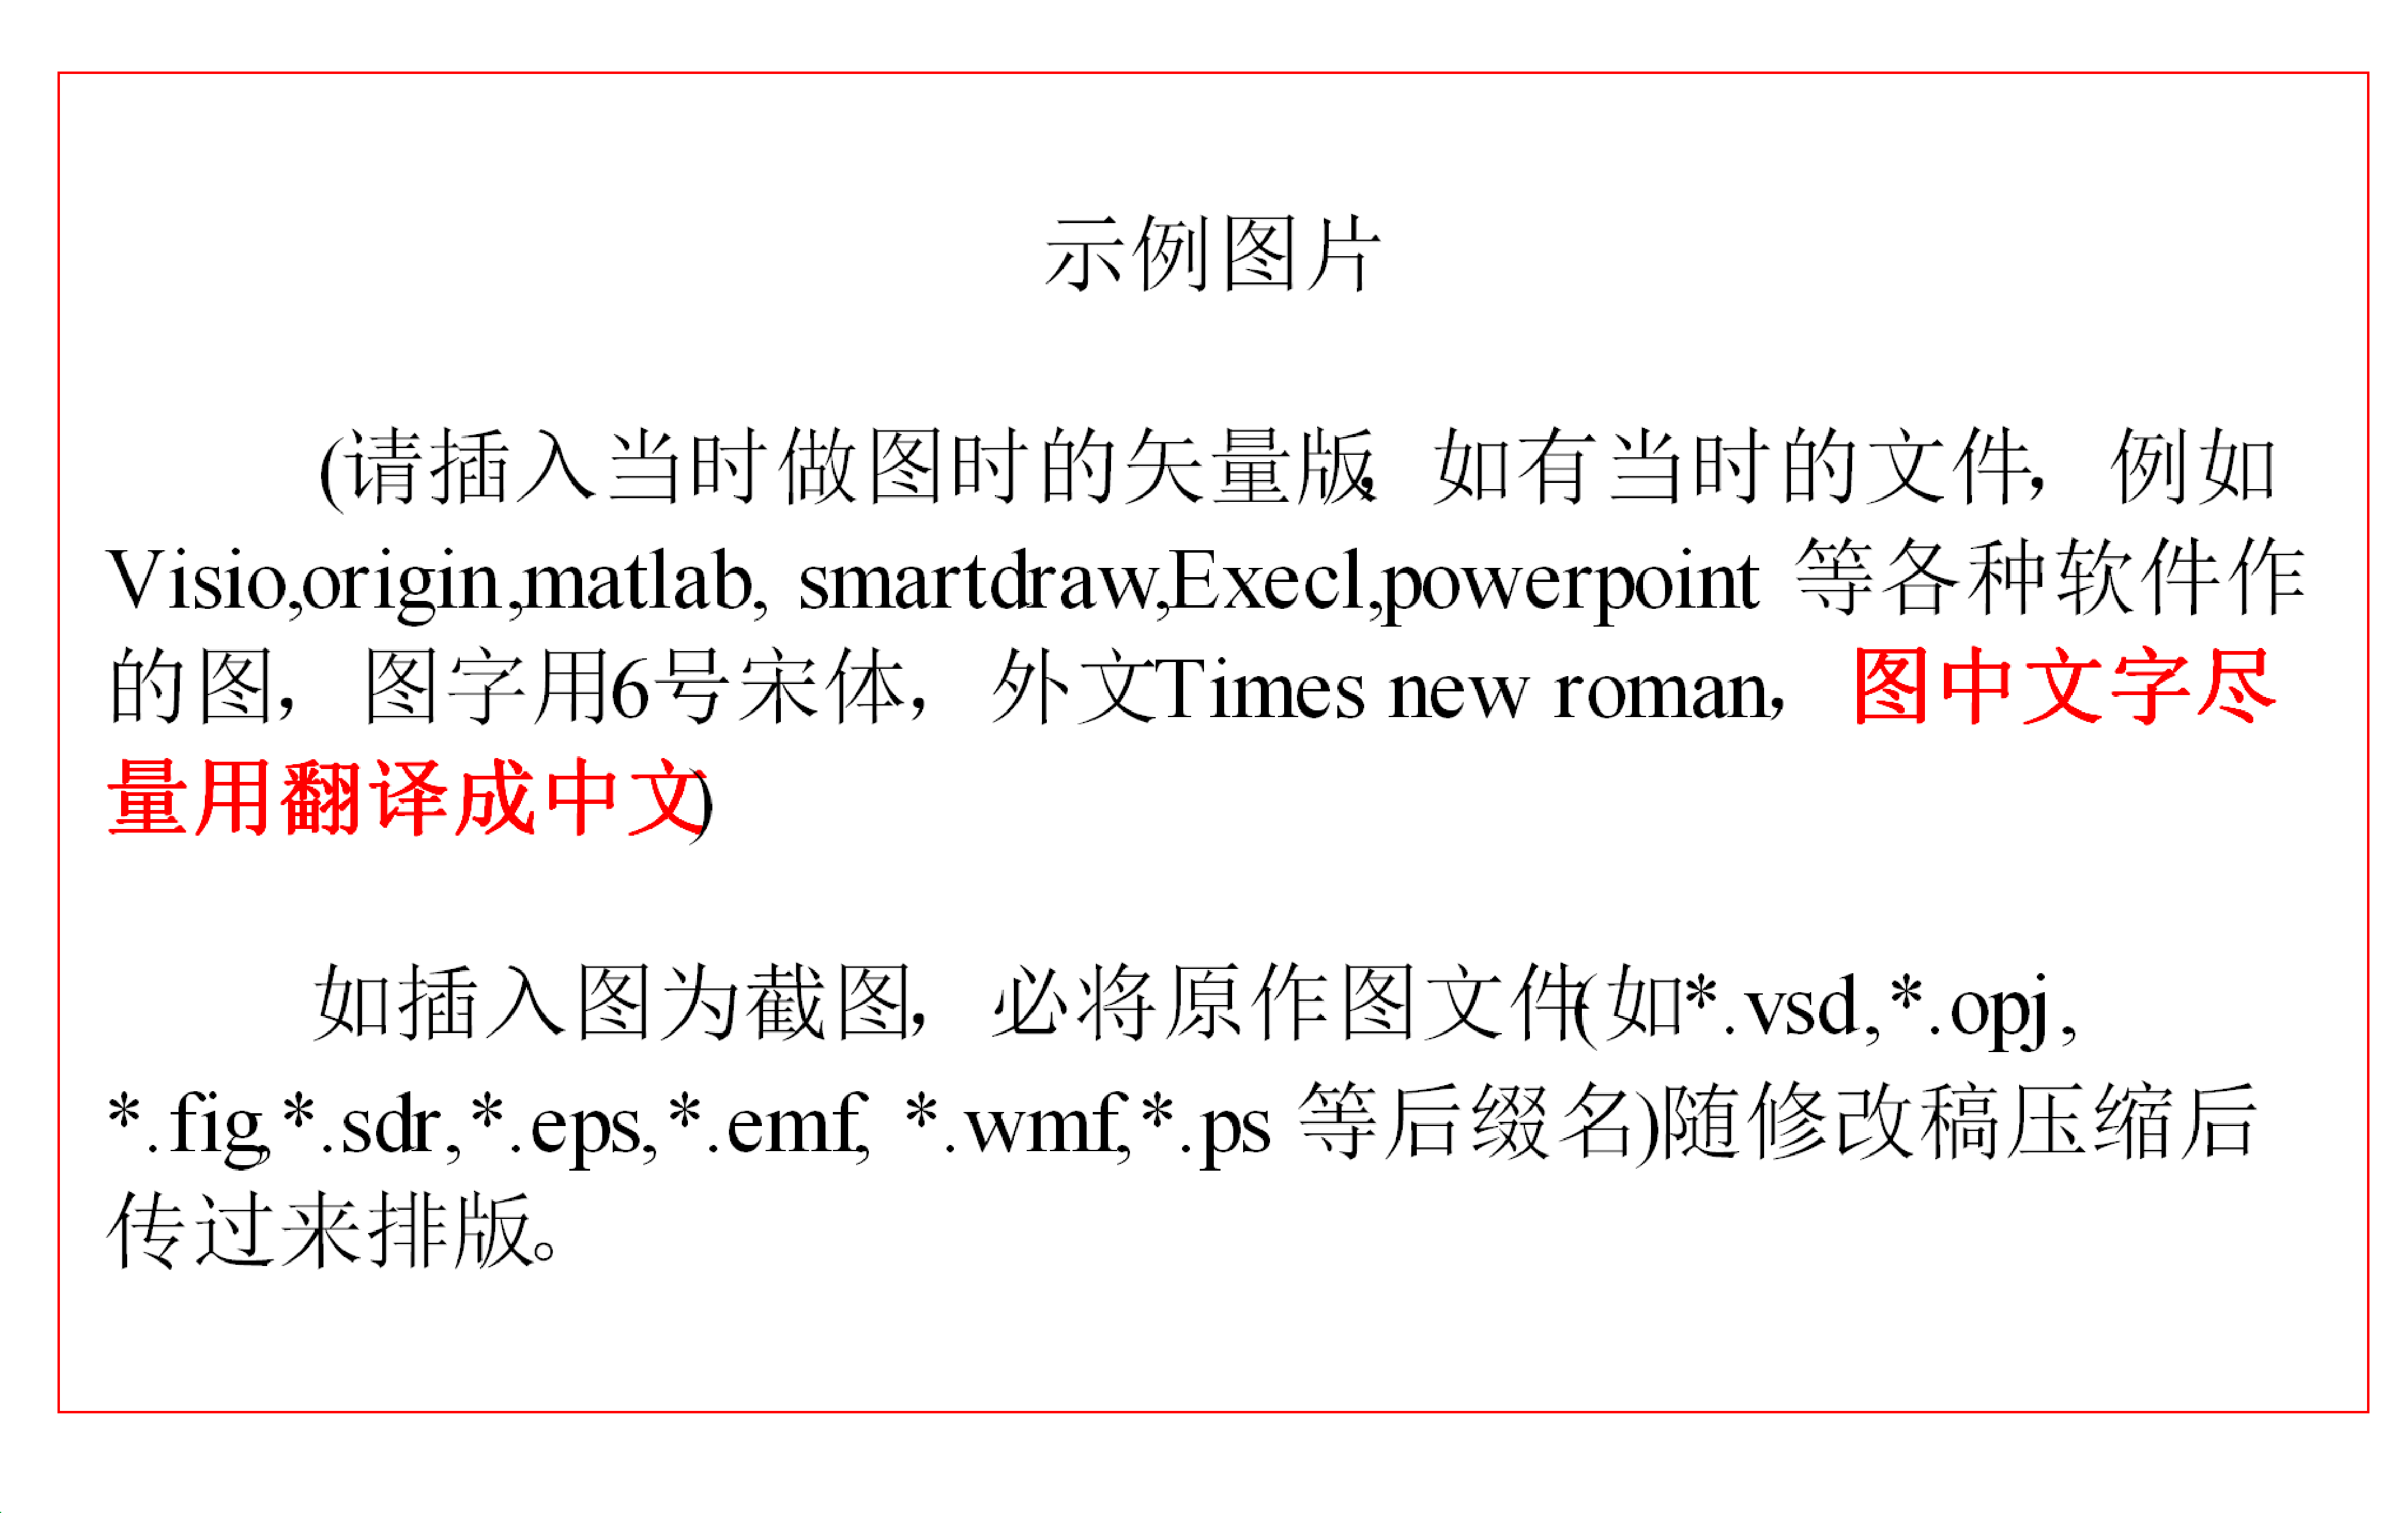
\includegraphics[width=3.15in,height=1.98in]{CJC1.pdf}}
图X\quad  图片说明 *字体为小5号,图片应为黑白图,图中的子图要有子图说明*
\label{fig1}
\end{figure}

\begin{table}[htbp]
\centering {\begin{CJK*}{UTF8}{zhhei}表X\quad 表说明 *表说明采用黑体*\end{CJK*}}
\vspace {-2.5mm}
\begin{center}
\begin{tabular}{ll}
\toprule
*示例表格*&*第1行为表头,表头要有内容* \\
\hline
&
 \\
&
 \\
&
 \\
&
 \\
\bottomrule
\end{tabular}
\label{tab1}
\end{center}
\end{table}

\begin{CJK*}{UTF8}{zhhei}过程X.\end{CJK*}\quad 过程名称

{\zihao{5-}*《计算机学报》的方法过程描述字体为小5号宋体,IF、THEN等伪代码关键词全部用大写字母,变量和函数名称用斜体*}


\begin{CJK*}{UTF8}{zhhei}算法\textbf{Y}\end{CJK*}.\quad 算法名称.
\zihao{5-}{

\noindent 输入:{\ldots} {\ldots}

\noindent 输出:{\ldots} {\ldots}

*《计算机学报》的算法描述字体为小5号宋体, IF、THEN等伪代码关键词全部用大写字母,变量和函数名称用斜体*}

\vspace {3mm}
\zihao{5}{
\noindent \begin{CJK*}{UTF8}{zhhei}致\quad 谢\end{CJK*}\quad \begin{CJK*}{UTF8}{kai} *致谢内容.* 致谢\end{CJK*}}


\vspace {5mm}
\centerline
{\zihao{5}
\begin{CJK*}{UTF8}{zhhei}参~考~文~献\end{CJK*}}

\begin{thebibliography}{99}
\zihao{5-} \addtolength{\itemsep}{-1em}
\vspace {1.5mm}

\bibitem[1]{ref1}
Sui Y, Zhou M, Zhou M, et al. Table meets llm: Can large language models understand structured table data? a benchmark and empirical study[C]//Proceedings of the 17th ACM International Conference on Web Search and Data Mining. 2024: 645-654.
  \end{thebibliography}

\begin{strip}
\end{strip}

\noindent {\zihao{5}\bf{附录X}.}

{\zihao{5-}\setlength\parindent{2em}
*\textbf{附录内容}置于此处,字体为小5号宋体。附录内容包括:\textbf{详细的定理证明、公式推导、原始数据}等*}

\begin{strip}
\end{strip}

\begin{biography}[yourphotofilename.jpg]
\noindent
\textbf{First A. Author}\ \ *计算机学报第1作者提供照片电子图片,尺寸为1寸。英文作者介绍内容包括:出生年,学位(或目前学历),职称,主要研究领域(\textbf{与中文作者介绍中的研究方向一致}).*
*字体为小5号Times New Roman*

\end{biography}

\begin{biography}[yourphotofilename.jpg]
\noindent
\textbf{Second B. Author} *英文作者介绍内容包括:出生年,学位(或目前学历),职称,主要研究领域(\textbf{与中文作者介绍中的研究方向一致})。*
*字体为小5号Times New Roman*
\end{biography}
\begin{strip}
\end{strip}
\zihao{5}
\noindent \textbf{Background}

\zihao{5-}{
\setlength\parindent{2em}
*论文背景介绍为\textbf{英文},字体为小5号Times New Roman体*

论文后面为400单词左右的英文背景介绍。介绍的内容包括:

本文研究的问题属于哪一个领域的什么问题。该类问题目前国际上解决到什么程度。

本文将问题解决到什么程度。

课题所属的项目。

项目的意义。

本研究群体以往在这个方向上的研究成果。

本文的成果是解决大课题中的哪一部分,如果涉及863$\backslash
$973以及其项目、基金、研究计划,注意这些项目的英文名称应书写正确。}

\end{CJK*}
\end{document}


